\documentclass[10pt,conference,compsocconf]{IEEEtran}

\usepackage{hyperref}
\usepackage{graphicx}	% For figure environment


\begin{document}
\title{Machine Learning Project 1 - Higgs Boson}

\author{
  Sami Ben Hassen, Firas Kanoun, Ali Fessi \\
  \textit{CS-433 Machine Learning, EPFL, Switzerland}
}

\maketitle

\begin{abstract}
  With faster and more powerful processors, Machine learning has become very important and offers useful tools and techniques to deal with a lot of problems in almost every scientific field.
  Regression is perhaps one of the most well-known and well understood algorithms in statistics and machine learning.
  In this paper we explore different types of regression and how they deal with a real life data-set from CERN in the field of physics.
\end{abstract}

\section{Introduction}

The Higgs boson is an elementary particle in the Standard Model of particle physics, produced by the quantum excitation of the Higgs field, one of the fields in particle physics theory~\cite{higgsboson}. 

The aim of this project is to distinguish between Higgs Boson and background noise. We started with a data-set that had 30 features describing a proton collision event. Through data cleaning and feature engineering we sought to remove the noise and implement machine learning methods to solve this binary classification problem.
\section{Models and Methods}
\label{sec:structure-paper}
\subsection{Mandatory algorithms implementation}
This project is part of a machine learning course, so before we dive in any predicting, we had the task to implement 6 machine learning algorithms presented in the lecture notes~\cite{MLepfl}.
Depicted in Table \ref{tab:initial_test} are the results we got after the implementation without any data cleaning nor feature engineering, the parameters chosen by hand without any optimization and the results obtained after doing a random 80-20 split on the data.
\begin{table}[h!]
    \centering
    \begin{tabular}{|l|c|c|c|c|}
\hline
                              & \multicolumn{3}{c|}{Parameters}   &           \\
\multicolumn{1}{|c|}{Methods} & $\lambda$ & $\gamma$  & max\_iter. & Pred (\%) \\ \hline
Least Squares                 & -         & -         & -         & 74.3      \\ \hline
Gradient Descent              & -         & $10^{-7}$ & 2000      & 69.8      \\ \hline
Stochastic Gradient Descent   & -         & $10^{-7}$ & 1000      & 69.3      \\ \hline
Ridge Regression              & $10^{-5}$ & -         & -         & 74.3      \\ \hline
Logistic Regression           & -         & $10^{-6}$ & 3000      & 75.4     \\ \hline
Reg Logistic Regression       & $10^{-2}$         & $10^{-6}$ & 3000      & 75.4     \\ \hline
\end{tabular}
    \caption{Initial test of the algorithms we were asked to implement.}
    \label{tab:initial_test}
\end{table}

\vspace{-0.7cm}
The results we got are poor as expected but still better than a flip of a coin. We can see that all the methods are close in their accuracy. On the raw data-set the Logistic Regression methods work best, trailed by Least Squares and Ridge Regression while we found that The Gradient Descent methods were less accurate. This is pretty logical since Logistic Regression is made to deal with this kind of classification problem.

\subsection{Analysis of the data-set}
Once we took a closer look at the data-set, there were a couple of observations that grabbed our attention :
\begin{enumerate}
\item The values feature 22 takes are all in $\{0,1,2,3\}$.
\item The existence of NaN values.
\item The correlation between certain features (Figure ~\ref{fig:correlation_table})
\item Features that take unique values.
\item Features that behave as a 'Gaussian' once we apply certain mathematical functions on them.
\end{enumerate}

\begin{figure}[htbp]
  \centering
  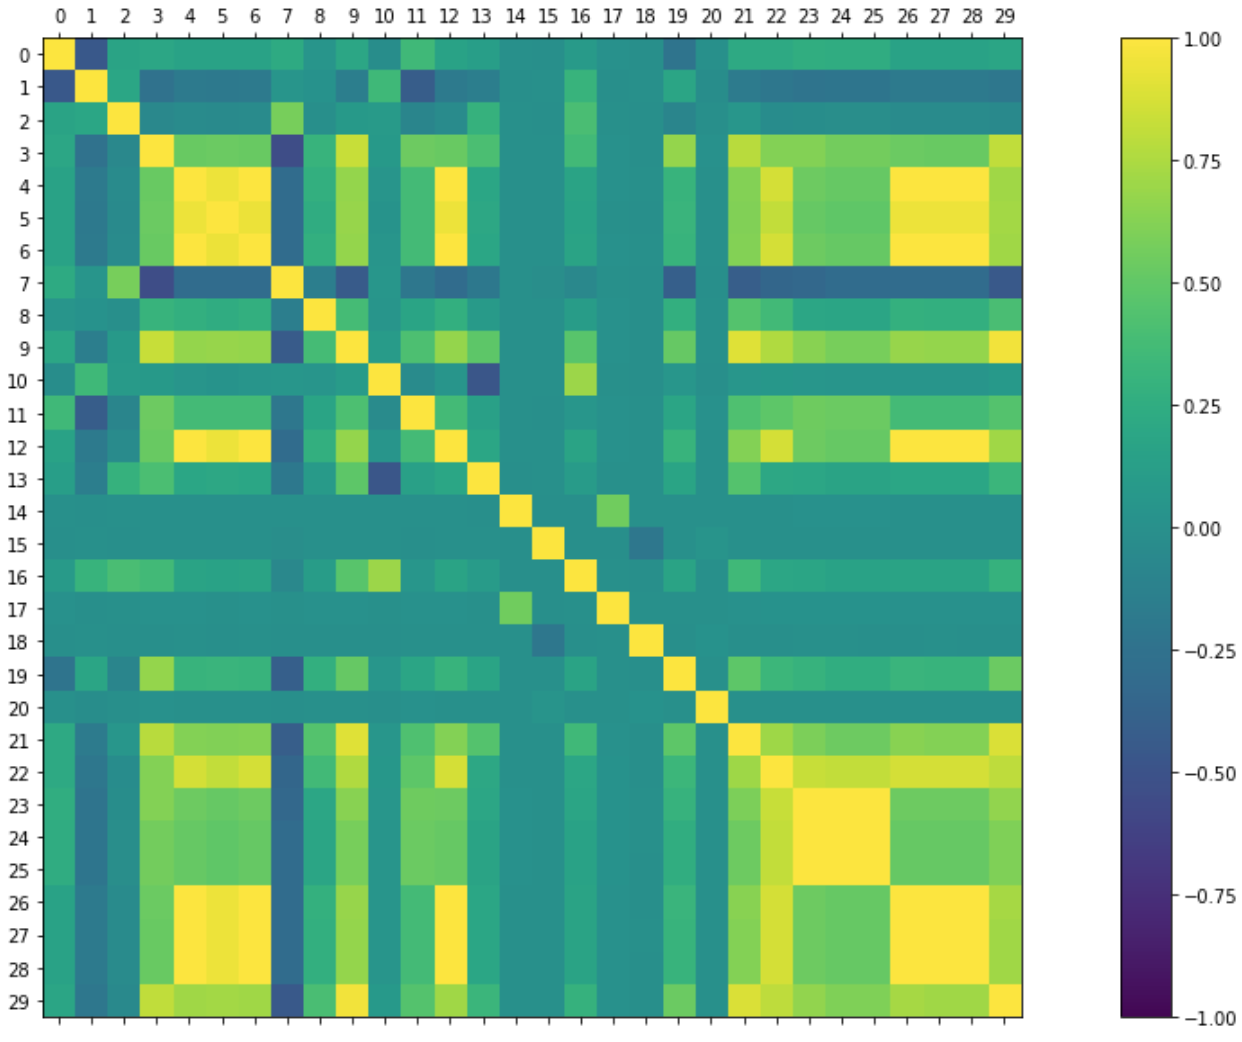
\includegraphics[width=\columnwidth]{latex-example-paper/CorrelationPlot.png}
  \vspace{-7mm}
  \caption{Correlation between different features (yellow means high correlation).}
  \vspace{-3mm}
  \label{fig:correlation_table}
\end{figure}
We decided to divide the data-set into 4 different subsets according to the values of column 22 that represent the jet number. Once we do that we notice that there were entire columns that take the value NaN or a unique value like 0 especially for jet 0 and jet 1. Getting rid of them was the only option.
After this, we moved on to the feature engineering task where we had to apply some uni-variate transforms to better expose the linear relationship between the inputs and the output~\cite{MLlogistic}. The transforms that worked the best for the different features were : \begin{enumerate}
\item The Logarithm function.
\item The Square root.
\item The Classification (Brings the values that are ranging between to 2 distinct extremes to discrete numbers).
\item Division by the absolute maximum.
\item Replacement of the NaN values by the mean.
\item Standardization.
\end{enumerate}
Fig~\ref{fig:feature_engineering_example} is a perfect example of how one can transform a certain feature.
\begin{figure}[htbp]
  \centering
  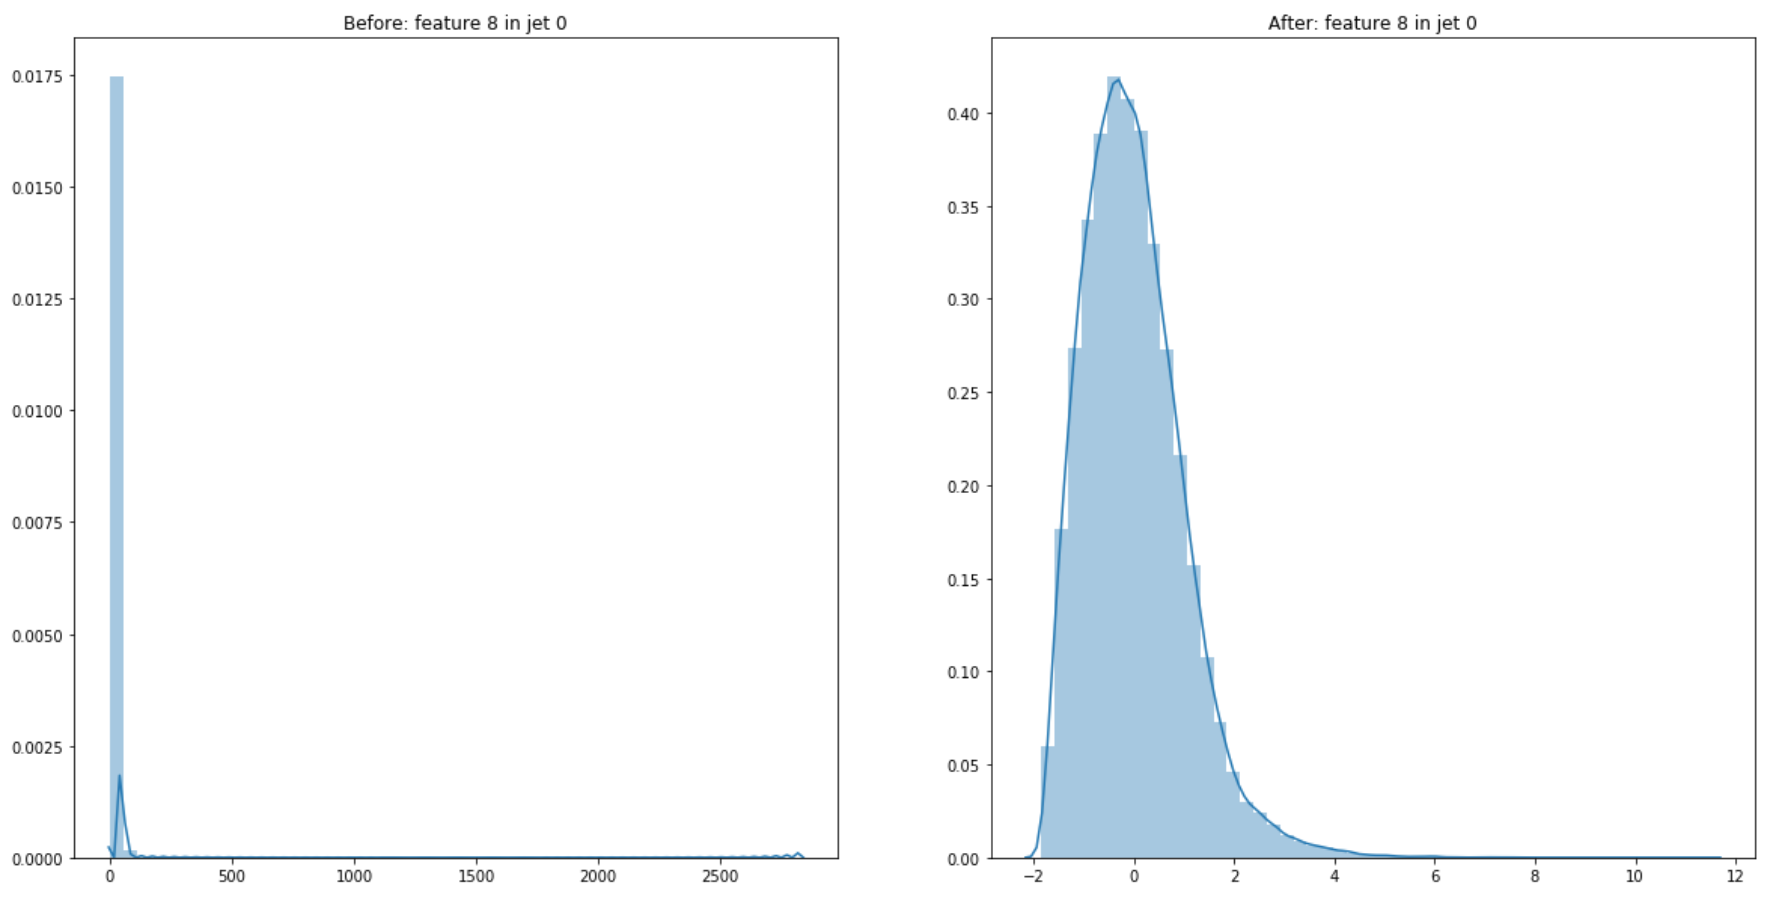
\includegraphics[width=\columnwidth]{latex-example-paper/feature_engineering.png}
  \vspace{-7mm}
  \caption{An example of a feature transformation.}
  \vspace{-3mm}
  \label{fig:feature_engineering_example}
\end{figure} 
\subsection{Cross validation}
Since we studied Logistic Regression very late, we tried to perfect the Ridge Regression method. To do this we used cross validation to find the best lambdas and degrees for each subset of the data-set. One example of a Cross Validation to find the lambdas is displayed in Figure~\ref{fig:cross_validation}.
\begin{figure}[htbp]
  \centering
  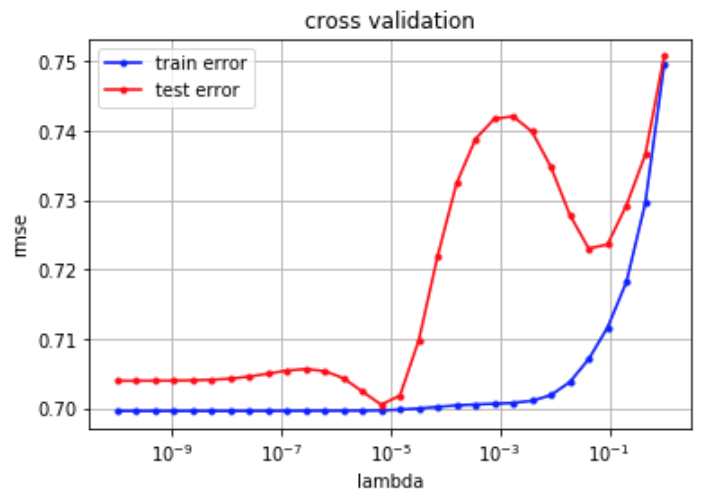
\includegraphics[width=\columnwidth]{latex-example-paper/cross_validation_example.png}
  \vspace{-7mm}
  \caption{Cross Validation for jet0 with degree 3 trying to locate best lambda).}
  \vspace{-3mm}
  \label{fig:cross_validation}
\end{figure}

\subsection{Adding features}
The above transformations helped us to clean the data-set but were not enough to get the best predictions. And that is why we have decided to add more features of our own:
\begin{itemize}
\item Apply the sine function.
\item Apply the cosine function.
\item Apply the exponential function.
\end{itemize}

We believe that these operations gave us more than enough features for our algorithm to find a linear relationship between the input and the output.

\subsection{Training}
Cross validation outputs the degrees and the $\lambda$s that guarantee the best loss in training without over-fitting.
We compute the new $X$ matrix using all the operations mentioned above along with the best degree. Then we apply the Ridge Regression algorithm with the best penalty $\lambda$ to find the best values for $W$
\subsection{Testing}
Once we get the optimal values for $W$ for each subset, We test our algorithm on all of them. the results are shown in Table \ref{tab:results_ridge}


\begin{table}[h!]
    \centering
    \begin{tabular}{c|c|c|c|c|c}
\cline{2-5}
\multicolumn{1}{l|}{}          & \multicolumn{4}{c|}{Subset by jet number} & \multicolumn{1}{l}{}         \\ \cline{2-6} 
                               & 0        & 1        & 2        & 3        & \multicolumn{1}{c|}{Overall} \\ \hline
\multicolumn{1}{|c|}{Accuracy (\%)} & 84.48    & 80.42    & 83.00    & 83.07    & \multicolumn{1}{c|}{82.75}   \\ \hline
\end{tabular}
    \caption{Results of Ridge Regression.}
    \label{tab:results_ridge}
\end{table}
\vspace{-0.7cm}
\section{Results and further discussion}

The predictive ability of the algorithms we were asked to implement was in accordance with what we have studied during this first half of the semester. However, due to a lack of time we couldn't perfect the parameters and the features to fully benefit from what Logistic Regression has to offer as the optimal method for binary classification. Nevertheless, the results that we managed to get show that Ridge Regression is as good.

With our way of feature engineering, Ridge Regression yielded an accuracy of 83\% on the Kaggle leaderboard dedicated to this class.

In hindsight, another way of cleaning the data could have been by splitting the data-set even more in order to get rid of the columns that had missing values. We could have even tried to predict them. However using the latter method could have been dangerous since we would be using values that are not 100\% correct in our models.

\section{Conclusion}
Through the course of this project, we implemented 6 methods of machine learning and we experienced hands-on the power and the limits of each one of them.

We learned how to explore the data, look for creative ways to clean it and get rid of all the missing values either by deleting the column if all it has are missing values or replacing them with the mean of the values of that feature.

\bibliographystyle{IEEEtran}
\bibliography{literature}

\end{document}
